\section{Results}
\label{sec:Results}

\fix{Nathan and Ron}

\begin{figure}[htb]
  \centering
  \includegraphics[width=\linewidth]{figures/MemoryUsageInSituPerNode.pdf}
  \caption{Plot of average per node memory usage of the in-situ run on Cielo.}
  \label{fig:MemoryInSituPerNode}
\end{figure}

\begin{figure}[htb]
  \centering
  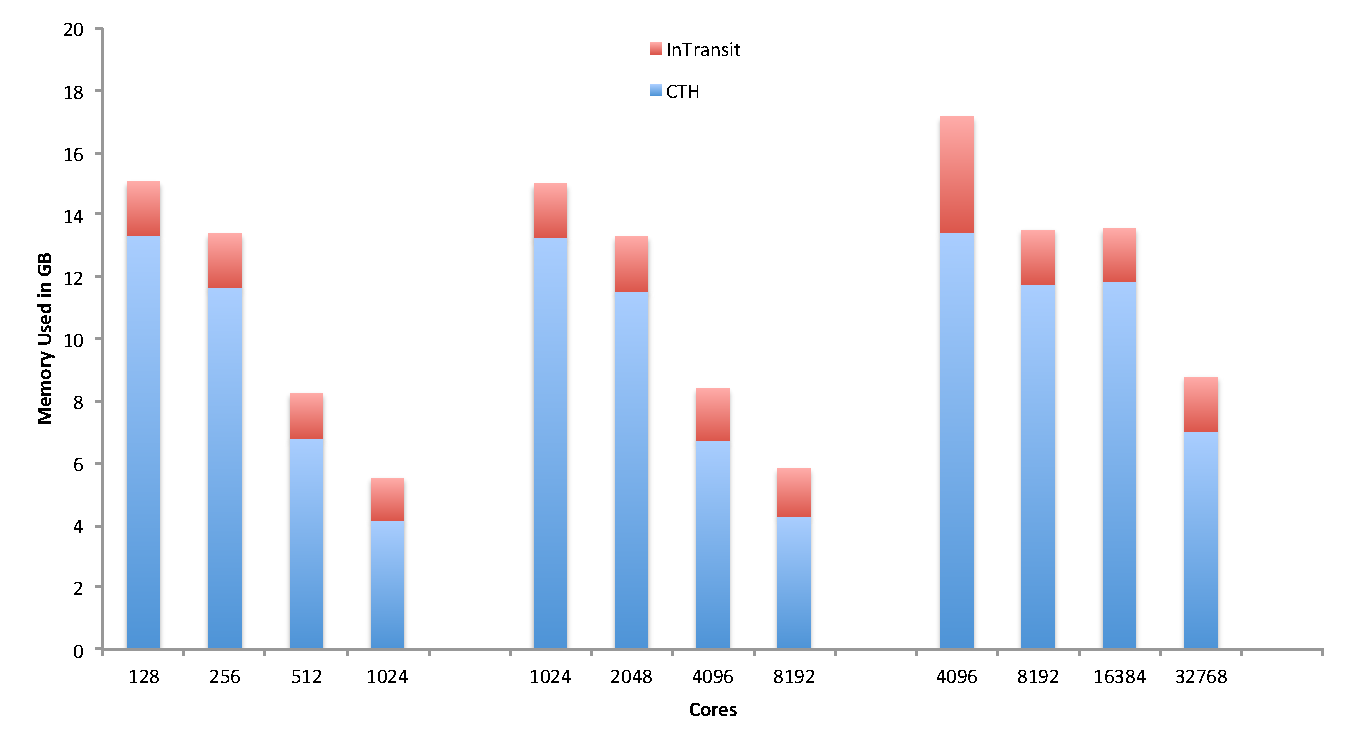
\includegraphics[width=\linewidth]{figures/MemoryUsageInTransitPerNode.pdf}
  \caption{Plot of average per node memory usage of the in-transit run on Cielo.}
  \label{fig:MemoryInTransitPerNode}
\end{figure}

\begin{figure}[htb]
  \centering
  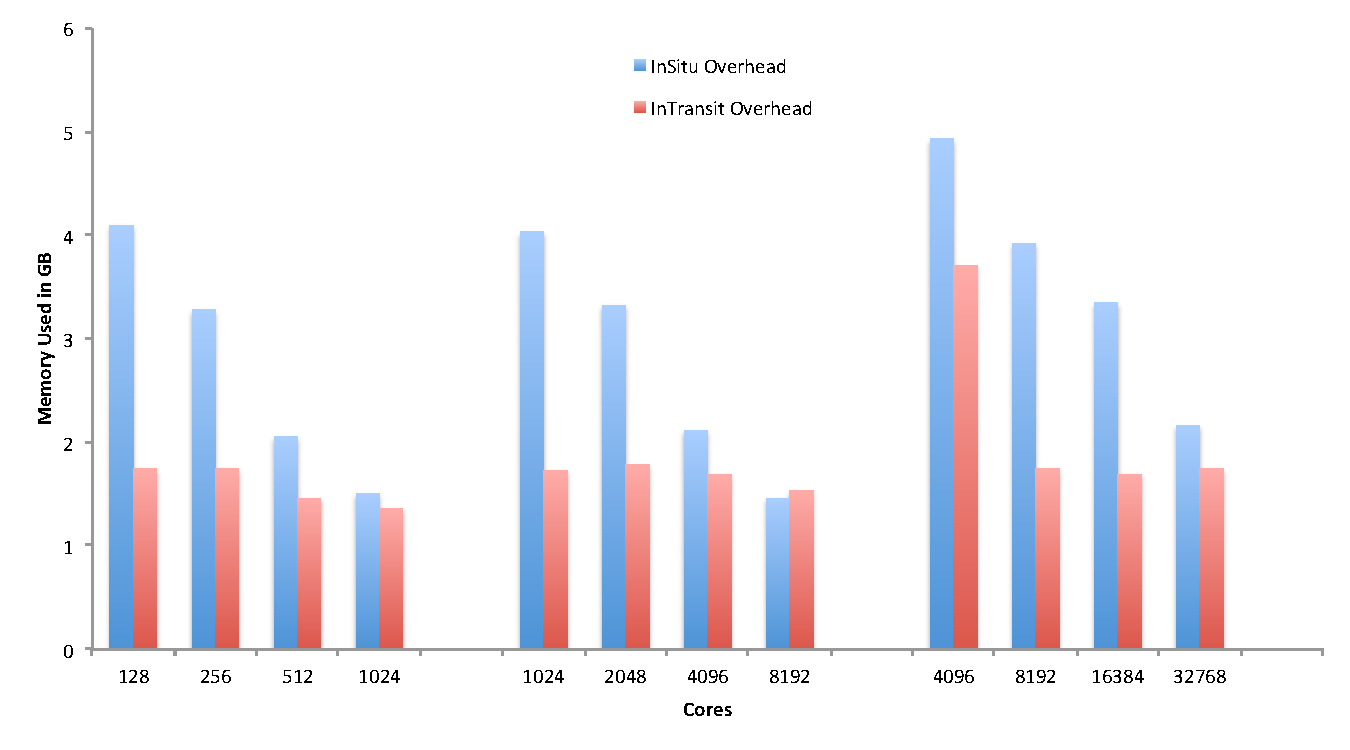
\includegraphics[width=\linewidth]{figures/MemoryUsageCompare.pdf}
  \caption{Plot of the average overhead per node of both InSitu and InTransit}
  \label{fig:MemoryCompare}
\end{figure}

\begin{figure}[htb]
  \centering
  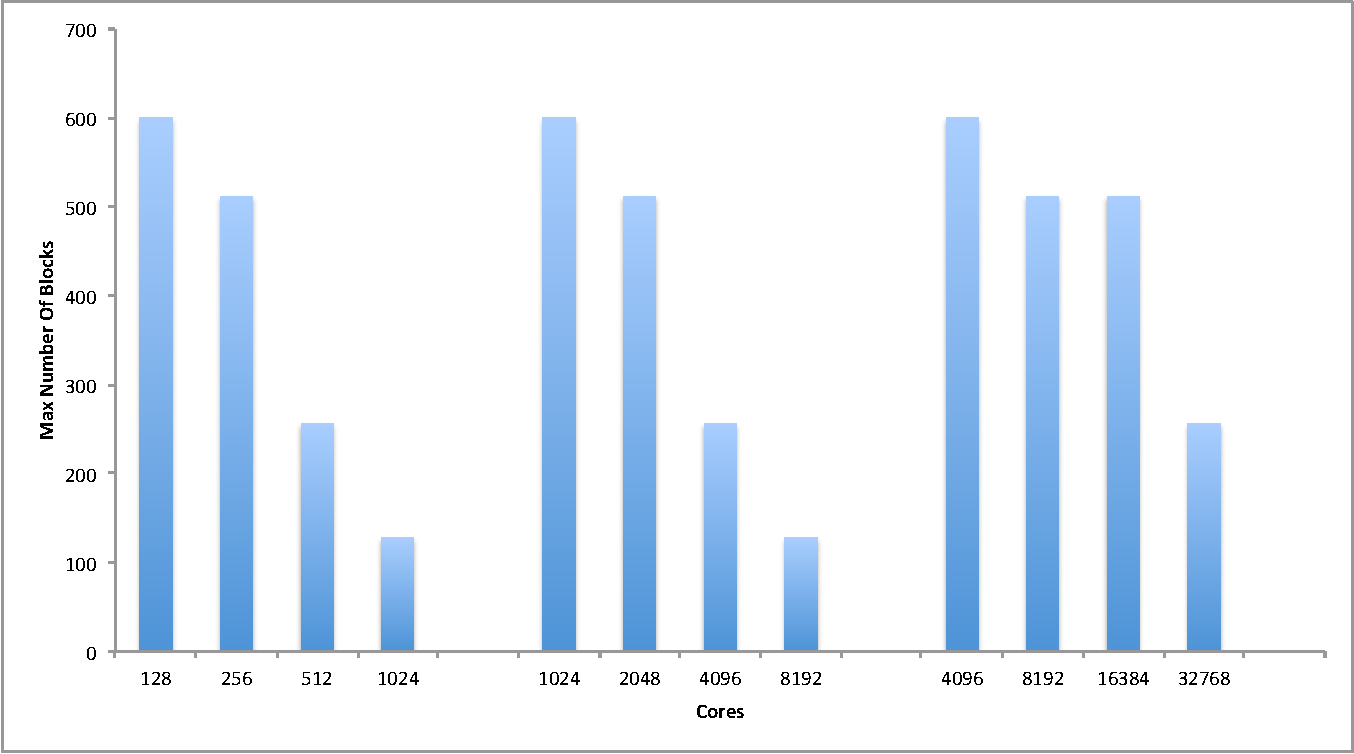
\includegraphics[width=\linewidth]{figures/MaxNumberOfBlocks.pdf}
  \caption{A plot of the "max number of blocks" parameter supplied to CTH for each run.}
  \label{fig:MaxBlocks}
\end{figure}

In order to under the CTH memory sizes, it is important to note that CTH
preallocates memory based on a value for "max number of blocks" provided
through the input deck.  Because of this, CTH memory usage is highly impacted
by the user specification.  In this case we ran the results with what we
believe are reasonable values for "max number of blocks" given the size of the
problem.  Figure~\ref{fig:MaxBlocks} shows the corresponding max blocks for
each run.


